% ICSE 2027 Tool Demonstration and Data Showcase
\documentclass[10pt,conference]{IEEEtran}
\usepackage[T1]{fontenc}
\usepackage{cite}
\usepackage{amsmath,amssymb}
\usepackage{graphicx}
\usepackage{booktabs}
\usepackage{xcolor}
\usepackage{tikz}
\usetikzlibrary{positioning,arrows.meta,fit,backgrounds}
\usepackage[hidelinks]{hyperref}

\newcommand{\tool}{STRATA}
\newcommand{\todo}[1]{\textcolor{red}{[TODO: #1]}}
\newcommand{\Dfull}{D}
\newcommand{\Dcut}{D_{\le t}}

\begin{document}

\title{\tool: Layer-by-Layer Point-in-Time Checking of\\ML Pipelines Written by Coding Agents}

\author{
\IEEEauthorblockN{Pavel Marian, Stanislav Chumakov, Danil Ezhov, Alexander Boukhanovsky}
\IEEEauthorblockA{AI Institute, ITMO University, Saint Petersburg, Russian Federation\\
\{pmarian, svchumakov\}@itmo.ru}
}

\maketitle

\begin{abstract}
We present \tool, a point-in-time checker for ML pipelines that coding
agents write over timestamped relational data. The tool runs
every layer of a pipeline (task, features, model, in-context examples,
agent) on the data as it is and as it was at the prediction time; any
difference in the layer's output is a LEAK witness that names the
time, entity, column and channel. A database enters only through an
availability schema, which \tool{} drafts from the raw files, with an
optional LLM agent for what column names do not say. On eight benchmark
databases \tool{} matches all 34 control verdicts and kills 43 of 43
point-in-time mutants with no false alarm on 55 harmless ones. On 134
generated feature programs it finds 16 leaks that a row-cut oracle misses,
and all 27 agent-written training runs on RelBench learn from rows after the
prediction time.
Demo: \url{https://jrzkaminski-strata-demo.static.hf.space}.
Video: \todo{video URL, e.g.\ \url{https://youtu.be/...}}
\end{abstract}

\begin{IEEEkeywords}
data leakage, point-in-time correctness, ML pipelines, coding agents, differential testing
\end{IEEEkeywords}

% ---------------------------------------------------------------------------
\section{Introduction}

Successful execution of an ML pipeline written by a coding agent does not
guarantee its temporal correctness. A pipeline that filters on one reference
timestamp can still read information that did not exist at the prediction
time, because availability is spread across tables, columns and the code
that trains the model. Such violations yield plausible features and inflated
offline results that do not reproduce at serving
time~\cite{kaufman2011,kapoor2023}. The property that every output computed
for time $t$ depends only on facts available at $t$ is called
point-in-time (PIT) correctness. Existing tools look at one place:
static analysis of notebook code~\cite{yang2022}, learned detectors over
code~\cite{peerj2025}, distribution checks in pipelines~\cite{mlinspect},
or single-feature AUC thresholds in AutoML products~\cite{datarobot,h2o}.
Feature frameworks offer cutoff times~\cite{dfs} but trust the user to know
when each value becomes known.

When an agent writes the whole pipeline, a leak can sit in any of five
layers: the task (which entities and labels exist at $t$), the
features, the model (which training rows it learns from), the
in-context (ICL) examples, and the agent itself (what it
recalls about known entities instead of reading the data). A check of one
layer passes a pipeline that leaks in another: agent-written scripts that
cut their features correctly still train on future labels
(Section~\ref{sec:eval}). Agents also meet databases nobody has annotated,
so a checker tied to one schema leaves them without a gate.

\tool{} closes this gap with one principle applied to every layer: a layer
is PIT-correct at $t$ if its output on the full database $\Dfull$ equals its
output on $\Dcut$, the database as it was at $t$. It contributes:
(i)~a database-agnostic oracle: a database enters only through an
availability schema of a few lines per table, which strata init
drafts from the raw files, optionally with an LLM agent, for review;
(ii)~five black-box layer checks with a verdict vocabulary that keeps
unknowns apart from passes and attaches a witness to every leak;
(iii)~agent integration: a CLI with exit codes and JSON reports, a
sandbox for code written by a model, and a skill file that a coding agent loads on
its own.

% ---------------------------------------------------------------------------
\section{The \tool{} Tool}

\begin{figure*}[t]
\centering
\resizebox{.8\textwidth}{!}{% STRATA workflow, drawn with TikZ so that the terms match the text.
% Input -> availability schema -> database states -> layer checks -> verdicts -> back to the agent.
% Needs \usetikzlibrary{positioning,arrows.meta,fit,backgrounds}.
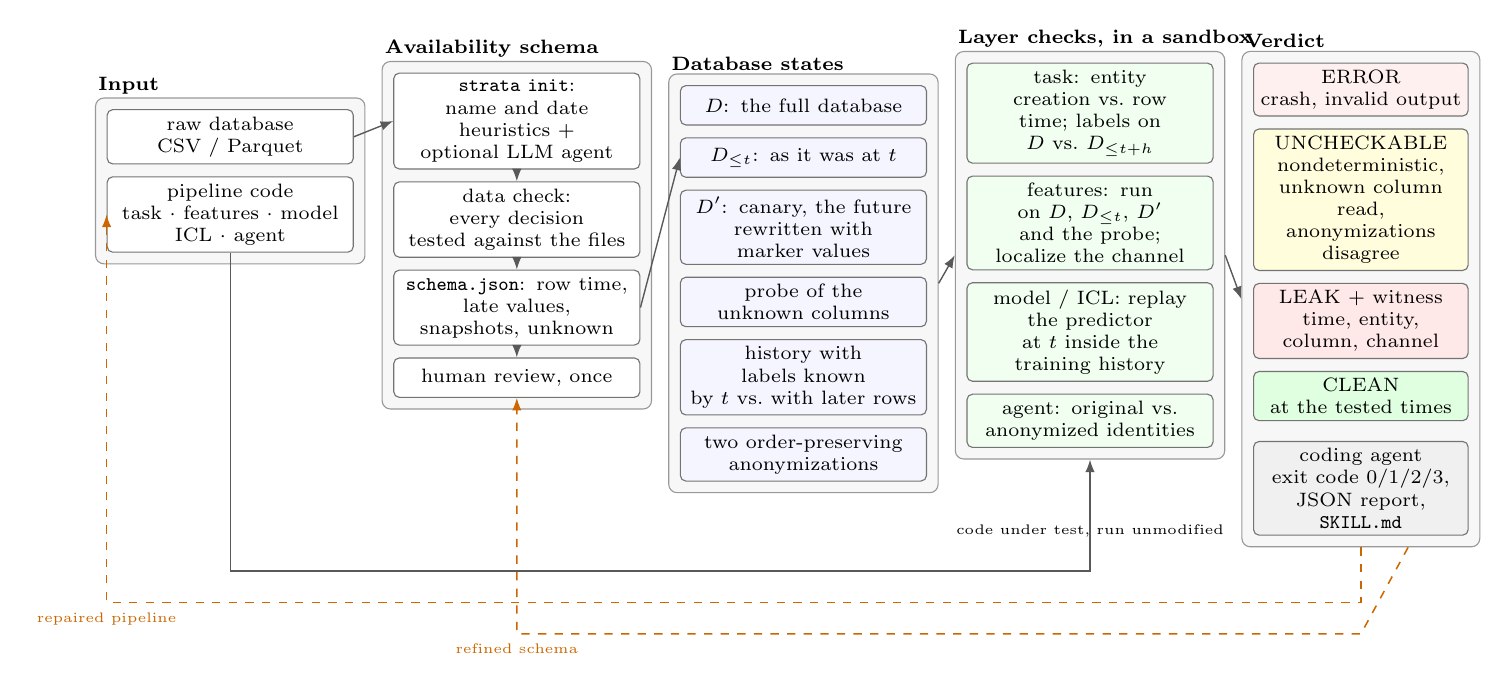
\begin{tikzpicture}[
  font=\scriptsize,
  every node/.append style={execute at begin node={\hyphenpenalty=10000 \exhyphenpenalty=10000 }},
  box/.style={draw=black!55, rounded corners=2pt, fill=white, align=center, inner sep=2.5pt, minimum height=5mm, text width=2.95cm},
  col/.style={draw=black!40, rounded corners=3pt, fill=black!3, inner xsep=4pt, inner ysep=4pt},
  head/.style={font=\scriptsize\bfseries, anchor=south west, inner sep=1pt},
  state/.style={box, fill=blue!4},
  check/.style={box, fill=green!6},
  verdict/.style={box, text width=2.55cm},
  arr/.style={-{Latex[length=1.6mm]}, draw=black!65, line width=.5pt},
  back/.style={-{Latex[length=1.6mm]}, draw=orange!80!black, line width=.55pt, dashed},
  node distance=1.5mm and 5mm]

% --- column 1: input
\node[box] (raw) {raw database\\CSV / Parquet};
\node[box, below=of raw] (code) {pipeline code\\task $\cdot$ features $\cdot$ model\\ICL $\cdot$ agent};

% --- column 2: availability schema
\node[box, right=of raw, yshift=2mm] (init) {\texttt{strata init}: name and date\\heuristics $+$ optional LLM agent};
\node[box, below=of init] (evid) {data check: every decision\\tested against the files};
\node[box, below=of evid] (schema) {\texttt{schema.json}: row time,\\late values, snapshots, unknown};
\node[box, below=of schema] (review) {human review, once};

% --- column 3: database states
\node[state, right=of init, yshift=2mm] (full) {$D$: the full database};
\node[state, below=of full] (cut) {$D_{\le t}$: as it was at $t$};
\node[state, below=of cut] (can) {$D'$: canary, the future\\rewritten with marker values};
\node[state, below=of can] (unk) {probe of the unknown columns};
\node[state, below=of unk] (hist) {history with labels known\\by $t$ vs.\ with later rows};
\node[state, below=of hist] (anon) {two order-preserving\\anonymizations};

% --- column 4: layer checks
\node[check, right=of full, yshift=-1mm] (ctask) {task: entity creation vs.\ row\\time; labels on $D$ vs.\ $D_{\le t+h}$};
\node[check, below=of ctask] (cfeat) {features: run on $D$, $D_{\le t}$, $D'$\\and the probe; localize the channel};
\node[check, below=of cfeat] (cmodel) {model / ICL: replay the predictor\\at $t$ inside the training history};
\node[check, below=of cmodel] (cagent) {agent: original vs.\\anonymized identities};

% --- column 5: verdicts
\node[verdict, right=of ctask, yshift=3mm, fill=red!6] (err) {ERROR\\crash, invalid output};
\node[verdict, below=of err, fill=yellow!14] (unch) {UNCHECKABLE\\nondeterministic, unknown column\\read, anonymizations disagree};
\node[verdict, below=of unch, fill=red!9] (leak) {LEAK $+$ witness\\time, entity, column, channel};
\node[verdict, below=of leak, fill=green!12] (clean) {CLEAN\\at the tested times};
\node[verdict, below=of clean, fill=black!6, yshift=-1mm] (agent) {coding agent\\exit code 0/1/2/3, JSON report,\\\texttt{SKILL.md}};

% --- column frames and headings
\begin{scope}[on background layer]
  \node[col, fit=(raw)(code)] (c1) {};
  \node[col, fit=(init)(review)] (c2) {};
  \node[col, fit=(full)(anon)] (c3) {};
  \node[col, fit=(ctask)(cagent)] (c4) {};
  \node[col, fit=(err)(agent)] (c5) {};
\end{scope}
\node[head] at (c1.north west) {Input};
\node[head] at (c2.north west) {Availability schema};
\node[head] at (c3.north west) {Database states};
\node[head] at (c4.north west) {Layer checks, in a sandbox};
\node[head] at (c5.north west) {Verdict};

% --- forward arrows
\coordinate (bot) at (current bounding box.south);
\draw[arr] (raw.east) -- (init.west);
\draw[arr] (init) -- (evid);
\draw[arr] (evid) -- (schema);
\draw[arr] (schema) -- (review);
\draw[arr] (schema.east) -- (cut.west);
\draw[arr] (c3.east) -- (c4.west);
\draw[arr] (c4.east) -- (c5.west);
\draw[arr] (code.south) |- ([yshift=-3mm]bot -| c4.south) -- (c4.south) node[pos=.5, below, font=\tiny] {code under test, run unmodified};

% --- feedback from the agent
\draw[back] (c5.south) -- ([yshift=-7mm]bot -| c5.south) -| (code.west) node[pos=.5, below, font=\tiny, orange!80!black] {repaired pipeline};
\draw[back] ([xshift=6mm]c5.south) -- ([yshift=-11mm]bot -| c5.south) -| (review.south) node[pos=.5, below, font=\tiny, orange!80!black] {refined schema};
\end{tikzpicture}
}
\caption{STRATA workflow: the schema drafted from the raw files and reviewed
once, the database states derived from it, the layer checks that run the
code unmodified in a sandbox, and the verdict that goes back to the agent.}
\label{fig:arch}
\end{figure*}

\textbf{Availability schema.} The schema is the only input specific to a
database, and every check is only as good as it. Each table is timed
(a row exists from its time column on), inherits its time through a
key, or is static. Late-filled values are declared as
self-available (a delivery date is known at its own value) or with a
stamp of their own (value\_time: a rating is known at
rated\_at). A stamp may also be a fixed date or null: a
value stored as its state at the end of the data (a final status, a current price, a
career total) is then never known before that date. Mutable columns whose
validity cannot be determined are unknown.
strata init drafts the schema from CSV or Parquet files: the
earliest date column becomes the row time, later date columns become
self-available, tables without dates inherit time through a shared key, and
text columns named like a status become unknown. Names and dates
do not reveal which values are snapshots taken at the end of the data, so strata init
-{}-llm adds a schema agent. An LLM (through OpenRouter) reads a profile of
the files, the heuristic draft and optional documentation, and returns every
decision with a reason in a fixed JSON schema; \tool{} checks each decision
against the data (missing columns, unparsable or late row times, broken
inheritance chains) and returns the findings for at most two revisions. The
model never produces a verdict or code.

\textbf{Database states.} For any $t$, $\Dcut$ removes rows that did not
exist and blanks values not yet filled. Some channels survive truncation,
so the canary $\Dfull'$ keeps $\Dcut$ intact but rewrites everything $\Dcut$
removes with marker values (shifted numbers, dates beyond the data horizon,
a reserved category). The unknown probe perturbs only unknown columns; keys
are never perturbed.

\textbf{Layer checks} (Fig.~\ref{fig:arch}). The lower bound of the
label check targets windows closed at $t$: events stamped exactly at $t$
move a microsecond into the past, so history is unchanged but such a window
loses them. Any pipeline function $f(db, ids, t)$, including a training
routine that builds its own examples, is checked like features, and a
feature leak is localized by cutting one channel at a time (rows of one
table, or one late-filled column) until the output changes. The model and
ICL checks replay a predictor at a query time inside the training history;
a label counts as known at $t$ when its row time plus the label horizon $h$
is at most $t$. The agent check needs two anonymizations, not
one. Both preserve order and equality, so a model that learns only from the
data cannot tell them from the original identities: real identities that
change the output signal recall or an external lookup, while anonymizations
that disagree with each other reveal a dependence on how identities are
spelled (hashed ID features) and yield UNCHECKABLE instead of a
false alarm.

\textbf{Verdicts.} The verification is one-sided: LEAK is a finite
witness of a violation, CLEAN only says that none was observed at the
times tested, and neither UNCHECKABLE nor ERROR counts as clean. Each
predictor is first replayed twice on identical input to detect
nondeterminism.

\textbf{Agent integration.} Every check is one command with exit code
0/1/2/3 for CLEAN/LEAK/UNCHECKABLE/ERROR
and a JSON report whose witness names the time, entity, column and channel.
Code under test runs in a forked child with a timeout, a memory limit and an
environment stripped of API keys. A SKILL.md file says when to call
which check, how to read a witness, that only a rerun may declare a leak
fixed, and that CLEAN is not a proof. The checker is about 1{,}300 lines of
Python on pandas with 38 tests; the examples for all ten databases differ
only in schema files and command templates.

% ---------------------------------------------------------------------------
\section{Demonstration}

\begin{figure}[t]
\centering
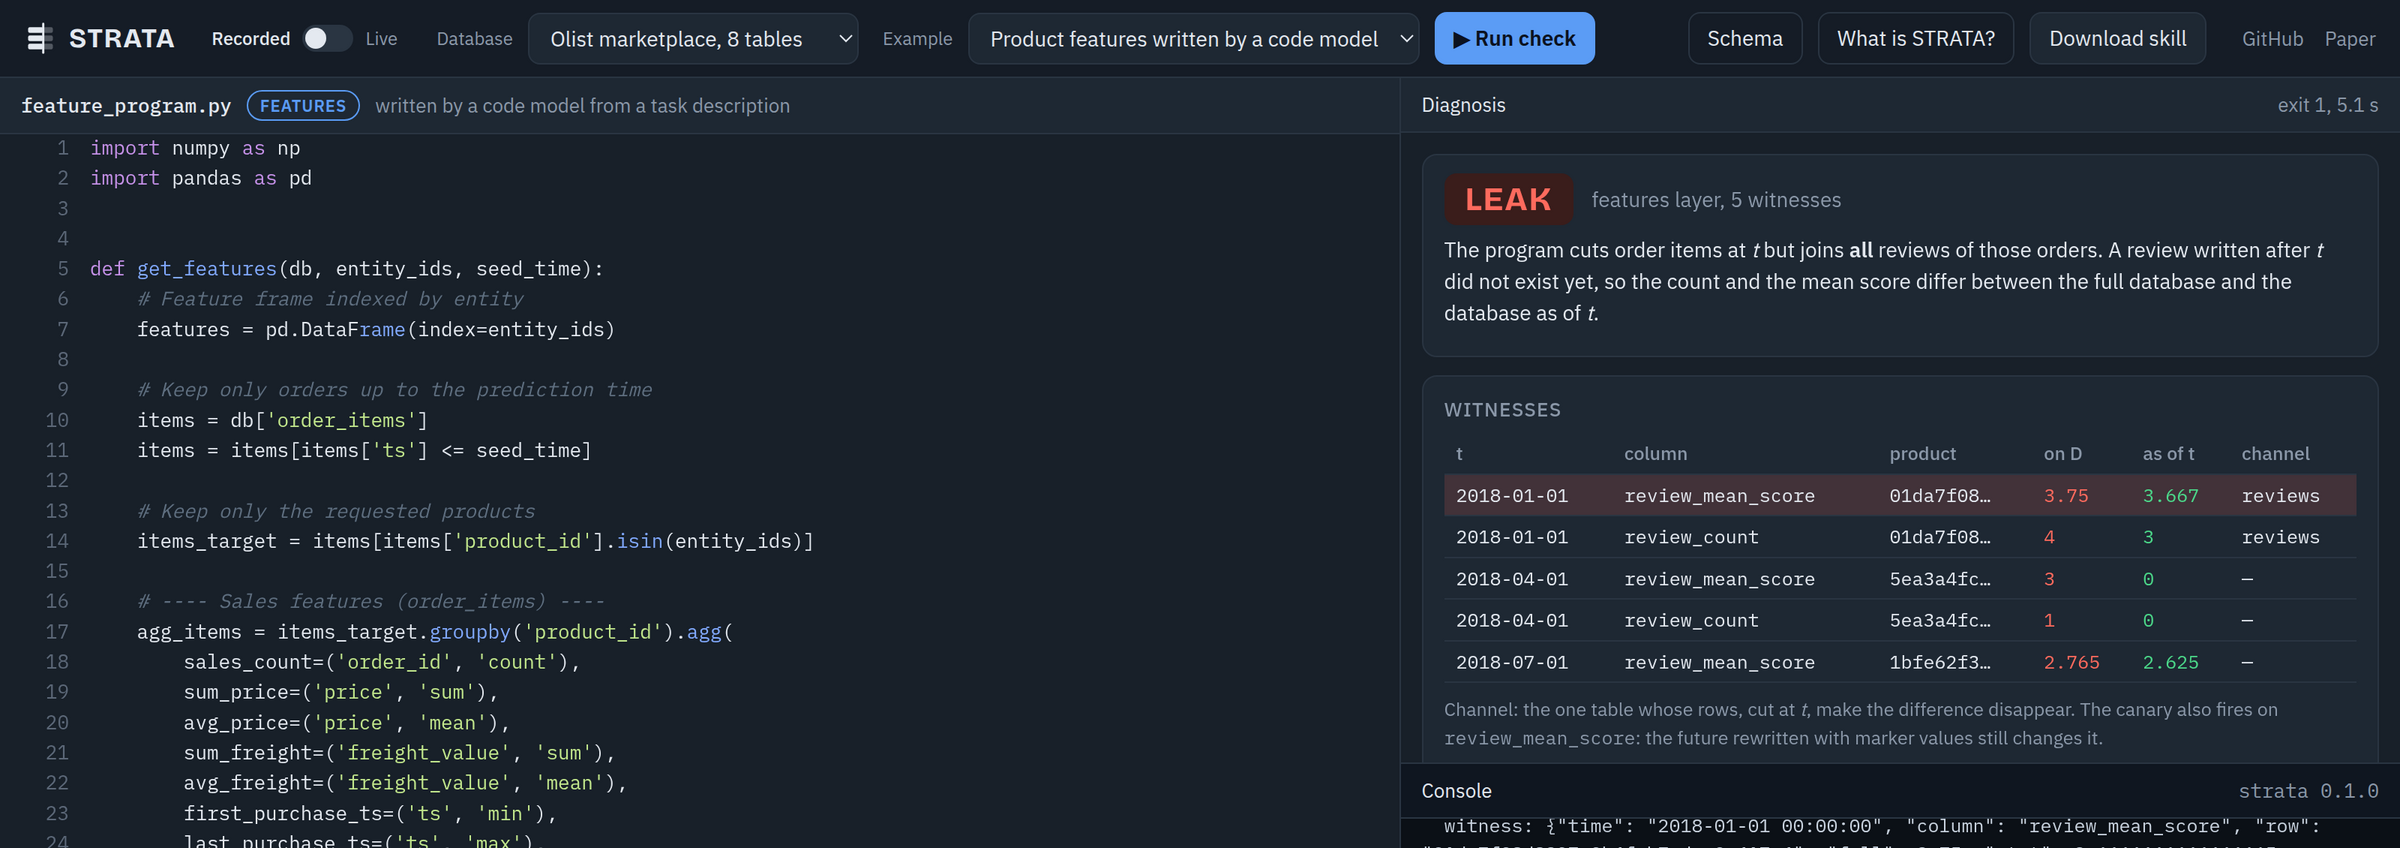
\includegraphics[width=.86\columnwidth]{demo_workbench.png}
\caption{The demo workbench on a recorded run: the program under test, the
verdict and its witnesses (time, product, both values, channel).}
\label{fig:demo}
\end{figure}

The demo is a browser workbench over recorded \tool{} runs on real data
(Fig.~\ref{fig:demo}). A feature program written by a code model for Olist
gets LEAK, localized to the reviews table, is repaired in place and rerun
CLEAN; a program that reads order\_status gets UNCHECKABLE with the output
columns that depend on it. The schema viewer shows the drafted Olist schema
with the LLM agent's reason per table. An agent-written
RelBench~\cite{relbench} script leaks in the model check; a second script
gets UNCHECKABLE in the identity check because its two anonymizations
disagree.
A second page runs \tool{} itself in the browser on a sample of Olist: a
model chosen by the viewer writes the program or drafts the schema from an
editable prompt, and the checks run on the result.

% ---------------------------------------------------------------------------
\section{Evaluation}
\label{sec:eval}

The experiments answer four questions, each backed by one table: does
\tool{} transfer across databases without code changes and separate
violations from harmless changes (Table~\ref{tab:pitbench}); is its verdict
more reliable than that of an oracle written for one database
(Table~\ref{tab:olist}); can the schema be drafted without hand annotation
(Table~\ref{tab:init}); and what does it find in training code written by
agents (Table~\ref{tab:relbench}).

\begin{table*}[t]
\centering\footnotesize
\setlength{\tabcolsep}{4.5pt}
\caption{One code base and one schema per database: \tool{} gets every
control verdict and separates violating from harmless mutants on all eight
PITBench databases, while each weaker detector fails on a different kind of
leak. Controls: leaking programs detected and correct programs flagged.
Mutants: behaviour-changing mutants, hand-labelled violations killed,
harmless mutants flagged. Leak classes: R rows not cut at
$t$, L late-filled value, S snapshot, A dump-time aggregate, B same-day
boundary, E entity before it exists, N neighbour statistic.}
\label{tab:pitbench}
\begin{tabular}{@{}llrl rrrr r rr rr@{}}
\toprule
& & & & \multicolumn{4}{c}{Controls} & \multicolumn{5}{c}{Mutants of the reference pipeline} \\
\cmidrule(lr){5-8}\cmidrule(l){9-13}
& & & & \multicolumn{2}{c}{\tool} & rows & + late & & \multicolumn{2}{c}{violations killed} & \multicolumn{2}{c}{harmless flagged} \\
\cmidrule(lr){5-6}\cmidrule(lr){10-11}\cmidrule(l){12-13}
Database & Domain & Rows & Classes & leaks & correct & cut & + canary & live & \tool & feat.\ only & \tool & any change \\
\midrule
Olist          & marketplace  & 0.94M & R L S       & 3/3 & 0/2 & 1/3  & 2/3  & 10 & 5/5   & 1/5  & 0/5  & 5/5   \\
F1             & sports       & 59k   & R B A       & 3/3 & 0/1 & 2/3  & 2/3  & 10 & 5/5   & 1/5  & 0/5  & 5/5   \\
PKDD'99        & banking      & 1.08M & R E L S S   & 5/5 & 0/1 & 2/5  & 2/5  & 15 & 6/6   & 1/6  & 0/9  & 9/9   \\
AdventureWorks & retail       & 174k  & R L S       & 3/3 & 0/1 & 1/3  & 2/3  & 13 & 5/5   & 1/5  & 0/8  & 8/8   \\
Northwind      & wholesale    & 3.2k  & R L S       & 3/3 & 0/1 & 1/3  & 2/3  & 14 & 6/6   & 1/6  & 0/8  & 8/8   \\
Sakila         & rental       & 39k   & R L S       & 3/3 & 0/1 & 1/3  & 2/3  & 10 & 5/5   & 1/5  & 0/5  & 5/5   \\
MovieTweetings & recsys       & 1.12M & R N         & 2/2 & 0/1 & 2/2  & 2/2  & 10 & 5/5   & 1/5  & 0/5  & 5/5   \\
TPC-H          & order entry  & 0.43M & R L S       & 3/3 & 0/1 & 1/3  & 2/3  & 16 & 6/6   & 1/6  & 0/10 & 10/10 \\
\midrule
Total          &              &       &             & 25/25 & 0/9 & 11/25 & 16/25 & 98 & 43/43 & 8/43 & 0/55 & 55/55 \\
\bottomrule
\end{tabular}
\end{table*}

\textbf{Eight databases (PITBench).} PITBench~\cite{pitbench} brings eight
relational databases to one contract: an availability map, 34 control
programs with known verdicts, and a reference pipeline per database. Each
map was translated into a \tool{} schema mechanically (time columns,
late-filled dates, snapshot columns as dated or null stamps), and
the controls ran unmodified at six times each. Table~\ref{tab:pitbench}
shows that a schema is all a new database needs: the verdicts do not depend
on the domain, size or leak classes, and the localized channel is the one
the control leaks through (rental.return\_date, product.list\_price). The
schema, in turn, decides what can be seen. Declaring the snapshot columns
unknown turns the 8 snapshot and aggregate controls into
UNCHECKABLE and changes nothing else; a naive F1 schema that times
results at midnight lets the leak at the race-day boundary pass as
CLEAN. A median control takes 2.6\,s.

\textbf{Mutants.} Five operators (remove a time cut, move a window past
$t$, widen the label horizon, swap </<=, remove a lower
bound) produce 144 mutants of the reference pipelines; the 98 that change
some output were labelled by hand as violations or not.
select\_entities, get\_features and fit\_predict
are checked like features, make\_label by the label check. In the
code and in the output, a harmless mutant (a longer window into the past, a
stricter cut) looks like a violation; only the comparison with the database
at $t$ tells them apart, on every database (Table~\ref{tab:pitbench}). Most violations sit outside the feature code: the training
routine fires in 32 kills and the label check in 19, and three kills need
the probe of the lower bound.

\textbf{Baselines} (Table~\ref{tab:pitbench}). Each weaker detector fails
on a different kind of leak, and the classes column shows which. Cutting
rows at $t$, as cutoff times in feature frameworks do, cannot see a value
filled in later or a snapshot, so it falls short exactly on the databases
with classes L and S; adding late-filled dates and a canary, as an oracle
for one database does, still misses every snapshot. The feature layer
alone misses the violations in label windows and training routines.
Treating any output change as a leak, as regression testing would, cannot
tell a violation from a harmless change. A static rule that flags code naming a late column or never
comparing with $t$, given the same schema, finds 22 leaking controls with 4
false alarms but only 6 violating mutants with 9 false alarms: a mutated
comparison still looks like a cut. The AutoML rule, a feature with AUC
above 0.85 (0.80), finds 4 (5) leaks and flags 3 of 9 correct programs:
leaked features need not be predictive, and good features are.

\textbf{Olist (features).} Corpus: the Olist e-commerce database and one
task, whether a product is ordered in the 90 days after $t$. Two code models
wrote 250 feature programs from a task description that never mentions
leakage; 134 execute. The reference is a handwritten oracle for Olist alone
that cuts rows by table time; both checkers ran with the same entities and
three prediction times. Table~\ref{tab:olist} shows that the two agree on
the oracle's leaks and part on its clean verdicts. The one leak \tool{}
does not confirm is a program truncated by the model's output limit, which
returns no frame. The programs the oracle wrongly passes filter orders by
purchase time but compute delivery times from delivery dates (15) or the
times of review answers (1) that were still in the future at $t$; a row
cut cannot see a value filled in later. Declared self-available in the
schema, these columns produce ordinary witnesses, so the canary adds no
further program. The UNCHECKABLE programs read
order\_status, which Olist overwrites without history; no oracle
can check them, and \tool{} says so instead of passing them.

\begin{table}[t]
\centering\footnotesize
\setlength{\tabcolsep}{4pt}
\caption{A CLEAN from an oracle written for one database is not
reliable: \tool{} confirms the oracle's leaks, but half of the programs the
oracle passes leak or cannot be checked. Rows: verdict of a handwritten
row-cut oracle on 134 generated programs.}
\label{tab:olist}
\begin{tabular}{@{}lrrrrl@{}}
\toprule
Row-cut oracle & LEAK & CLEAN & UNCH. & ERROR & Main channel \\
\midrule
LEAK (63)  & 62 & 0  & 0  & 1 & reviews rows \\
CLEAN (71) & 16 & 35 & 20 & 0 & delivery dates \\
\bottomrule
\end{tabular}
\end{table}

\begin{table}[t]
\centering\footnotesize
\setlength{\tabcolsep}{4pt}
\caption{Drafted schemas on the eight PITBench databases against the
hand-made maps, and the 34 controls run on the drafts. Names and dates
suffice except for snapshots, which the LLM agent finds. Caught and flagged
mean LEAK or UNCHECKABLE.}
\label{tab:init}
\begin{tabular}{@{}lrr@{}}
\toprule
& Heuristic & LLM agent \\
\midrule
Row times as in the map            & 18/26      & 23/26 \\
Late-filled dates found (extra)    & 12/14 (22) & 13/14 (19) \\
Snapshot columns caught            & 5/50       & 50/50 \\
\midrule
Leaking controls caught            & 23/25      & 25/25 \\
Verdict as expected                & 26/34      & 30/34 \\
Correct controls flagged           & 3/9        & 3/9 \\
\bottomrule
\end{tabular}
\end{table}

\textbf{Schema drafting} (Table~\ref{tab:init}). Schemas for the eight
PITBench databases were drafted from the raw files alone, with the
heuristics and with the agent (Claude Opus 5.5 without tool access, so the
maps could not be read). Snapshots decide the outcome: on the heuristic
drafts two F1 leaks (race-day boundary, career totals) pass as
CLEAN, on the agent's drafts none does. The heuristics take a wrong date as the row time
(the shipped date of Northwind orders, the date from which the PKDD'99
district statistics are known), and the missing rows look like a leak. The
agent's flags are cautious or deliberate: it declares two mutable columns
unknown (Northwind freight, Sakila payment amount), which gives
UNCHECKABLE, and it times Olist reviews by the customer's answer,
not by the survey date, since the score does not exist before the answer.
It kept that decision with a reason when the data check queried it and
listed it as a question for the data owner. A schema takes 1--3 calls, about
a minute per database; two runs differ in one decision.

\begin{table}[t]
\centering\footnotesize
\setlength{\tabcolsep}{2.6pt}
\caption{All 27 agent-written training runs on RelBench learn from rows
after $t$; the query AUC rises in only 5--6 of the 9 runs per task. AUC:
median, and runs in which it rises.}
\label{tab:relbench}
\begin{tabular}{@{}lrrrrrrrr@{}}
\toprule
& \multicolumn{2}{c}{Rows} & & \multicolumn{3}{c}{Query AUC} & \multicolumn{2}{c}{Identity} \\
\cmidrule(lr){2-3}\cmidrule(lr){5-7}\cmidrule(l){8-9}
Task & $\le t$ & $>t$ & $\max|\Delta s|$ & at $t$ & full & rises & CLEAN & UNCH. \\
\midrule
f1/dnf       & 7{,}729 & 3{,}650  & 0.04--0.86 & 0.91 & 0.95 & 6 & 6 & 3 \\
f1/top3      & 919     & 412      & 0.06--1.00 & 0.71 & 0.82 & 5 & 7 & 2 \\
event/ignore & 3{,}755 & 14{,}727 & 0.13--0.96 & 0.79 & 0.92 & 6 & 6 & 3 \\
\bottomrule
\end{tabular}
\end{table}

\textbf{RelBench (model and agent).} Three isolated sessions of one
commercial coding agent each wrote three training scripts for three binary
tasks (27 runs). \tool{} runs them unmodified through one command template,
with the official label horizons (30 days for F1, 7 for Event).
Every run is LEAK: the scripts train on the whole table they are given and never
bound it by the label horizon. The metric would not have revealed this: the
median AUC rises on every task, but not in 10 of the 27 runs, so the verdict
rests on the outputs. The identity check finds no
recall; its UNCHECKABLE runs come from three scripts whose outputs
differ between the two anonymizations (hashed or scaled ID features), and a
comparison of original and anonymized identities alone would report them
as recall.

\textbf{Cost.} On four cores a feature check of an Olist program takes a
median 6.5\,s, a model check of an agent script 5--6\,s.

\textbf{Limitations.} A schema is a claim about the data, and a verdict is
only as good as its schema; CLEAN is scoped to the tested times
and entities; the model and ICL checks need a time column and a declared
label horizon; the agent check detects identity dependence, not pretraining
as such; one base model wrote the RelBench corpus; the PITBench controls
and mutation labels have one annotator, and the agent and ICL checks have no
natural positives yet, so zero false alarms is an observation, not a bound;
the schema agent sends a profile with sample values to the model provider
(-{}-no-samples keeps them local).

% ---------------------------------------------------------------------------
\section{Related Work}

Temporal leakage is a recurring source of irreproducible ML
results~\cite{kaufman2011,kapoor2023}. Static detectors find leakage
patterns in notebooks~\cite{yang2022}, and learned models classify
code~\cite{peerj2025}; both judge code, whereas \tool{} judges outputs and
therefore treats model training and context assembly like features.
The verification is one-sided, as in look-ahead freedom as temporal
non-interference~\cite{fonseca2026}, a static formulation for one layer of
backtesting code. Featuretools cutoff times~\cite{dfs} prevent row leakage
when availability is given; \tool{} stamps values as well as rows.

% ---------------------------------------------------------------------------
\section{Availability}

Demo (project page, workbench, live run, usage instructions):
\url{https://jrzkaminski-strata-demo.static.hf.space}. Code, tests, the
schemas and replay scripts for Olist, RelBench and PITBench, run logs, the
27 agent-written scripts with replay inputs, and the skill file:
\todo{GitHub / Zenodo URL}, \todo{license}.

\bibliographystyle{IEEEtran}
\bibliography{refs}

\end{document}
